% begin module absolute-value 
\begin{frame}
\begin{example} %[Example 8, p. 18]
The absolute value $|a|$ of a number $a$ is defined to be
\[
|a| = \left\{ \begin{array}{ccccl}
\alert<handout:0| 2-3>{a} & \alert<handout:0| 3>{\textrm{if}} & \alert<handout:0| 3>{ a} & \alert<handout:0| 3>{\geq} & \alert<handout:0| 3>{0} \\
\alert<handout:0| 4-5>{-a} & \alert<handout:0| 5>{\textrm{if}} &  \alert<handout:0| 5>{a} & \alert<handout:0| 5>{<} & \alert<handout:0| 5>{0}. \end{array}\right.
\]

Sketch a graph of the function $f(x) = |x|$.

\begin{center}
\ \only<handout:0| 1>{%
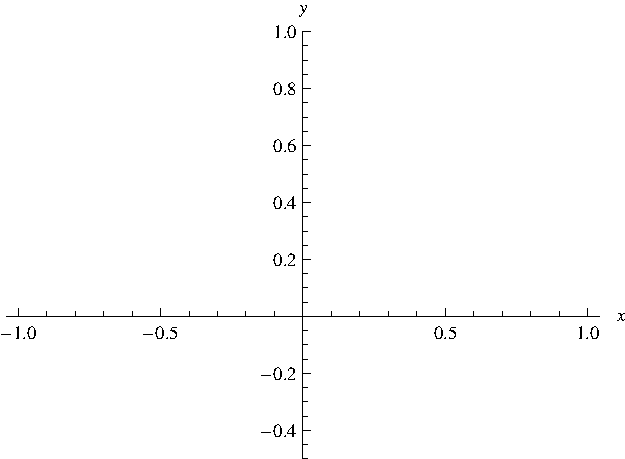
\includegraphics[height=4cm]{precalculus/pictures/01-01-ex-08a.pdf}%
}%
\only<handout:0| 2>{%
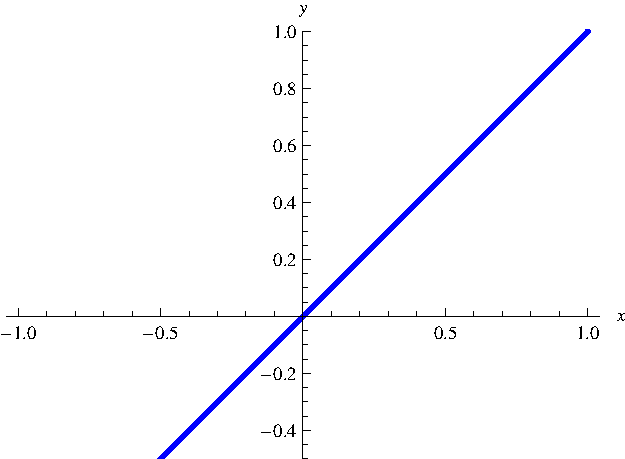
\includegraphics[height=4cm]{precalculus/pictures/01-01-ex-08b.pdf}%
}%
\only<handout:0| 3>{%
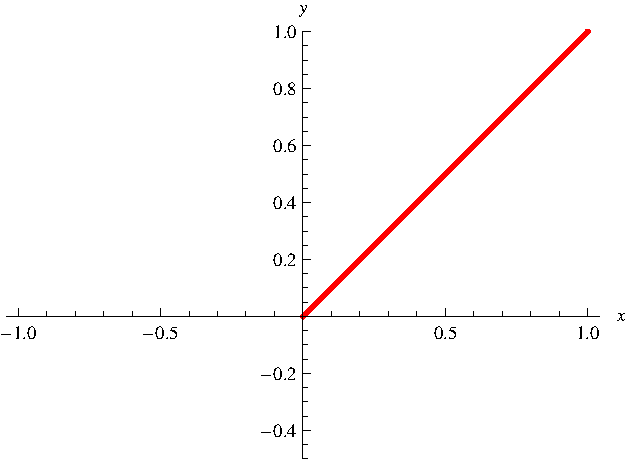
\includegraphics[height=4cm]{precalculus/pictures/01-01-ex-08c.pdf}%
}%
\only<handout:0| 4>{%
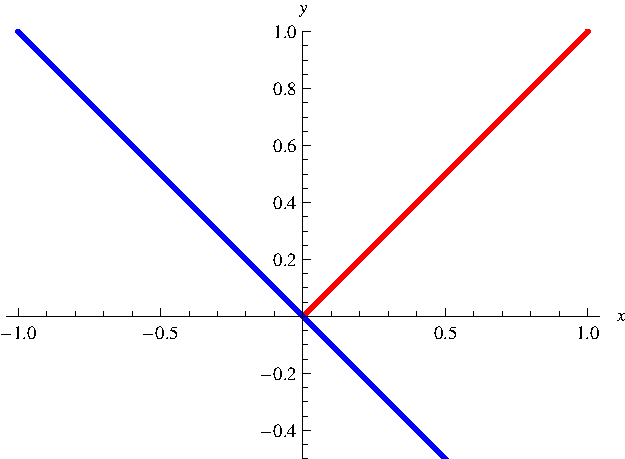
\includegraphics[height=4cm]{precalculus/pictures/01-01-ex-08d.pdf}%
}%
\only<handout:1-| 5>{%
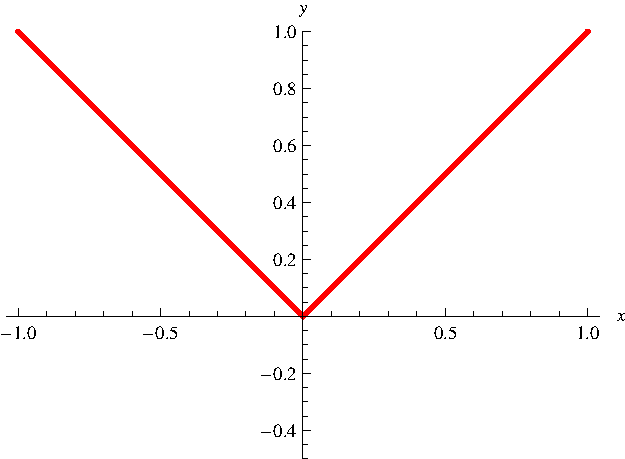
\includegraphics[height=4cm]{precalculus/pictures/01-01-ex-08e.pdf}%
}%
\end{center}
\end{example}
\end{frame}
% end module absolute-value 
